\documentclass[aspectratio=169,usenames,dvipsnames]{beamer}

\usetheme{default}  % You can choose any other theme you prefer

\title{04 - Algoritmos}
\author{Mateus Oliveira de Figueiredo}
\date{26/09/2023}

\usepackage{tikz}
\usepackage{multicol}
\usepackage{algorithm}
\usepackage{algpseudocode}
\usepackage{xcolor}
\usepackage[utf8]{inputenc}

\usepackage{pgfplots}
\DeclareUnicodeCharacter{2212}{−}
\usepgfplotslibrary{groupplots,dateplot}
\usetikzlibrary{patterns,shapes.arrows, positioning}
\pgfplotsset{compat=newest}

\begin{document}

\begin{frame}
\titlepage
\end{frame}

\begin{frame}
\frametitle{Problema}

\onslide<1->{
    Dado um conjunto de pontos no  $\mathbb{R}^2$, encontrar o menor conjunto convexo que contém todos os pontos (fecho convexo).
}
\begin{figure}
\begin{overprint}
  \onslide<1> \begin{center}
% This file was created with tikzplotlib v0.10.1.
\begin{tikzpicture}[scale=0.9]

\definecolor{darkslategray38}{RGB}{38,38,38}
\definecolor{lightgray204}{RGB}{204,204,204}
\definecolor{steelblue76114176}{RGB}{76,114,176}

\begin{axis}[
axis line style={lightgray204},
hide x axis,
hide y axis,
tick align=outside,
x grid style={lightgray204},
xmajorticks=false,
xmin=0.0669367338947019, xmax=0.894111789939664,
xtick style={color=darkslategray38},
y grid style={lightgray204},
ymajorticks=false,
ymin=-0.0362471743023485, ymax=1.03274876525929,
ytick style={color=darkslategray38}
]
\addplot [draw=steelblue76114176, fill=steelblue76114176, mark=*, only marks]
table{%
x  y
0.346517060199814 0.201667385571862
0.110198245014805 0.710446973195645
0.674196381095166 0.49152149407659
0.30956117598126 0.80506608165215
0.271019344924566 0.98415804073376
0.636154602711755 0.693008958661624
0.384544745815431 0.621686927298183
0.613069361293463 0.536676532843469
0.515872695614497 0.0123435502231805
0.856512923755802 0.429885536698643
0.794765500051758 0.575905243509799
0.104535600078564 0.331190264339077
0.698107527894101 0.591287819523784
0.652331867510728 0.829843579751645
0.776100950068952 0.0753407526360956
0.359461819254946 0.832493157115646
0.234215740614521 0.440279847038206
0.474800803395323 0.180277096021146
0.478504950884847 0.867281705269675
0.434092000130053 0.504691515965982
0.640277876553855 0.402360080889356
};
\end{axis}

\end{tikzpicture}

\end{center}
  \onslide<2> % This file was created with tikzplotlib v0.10.1.
\begin{center}
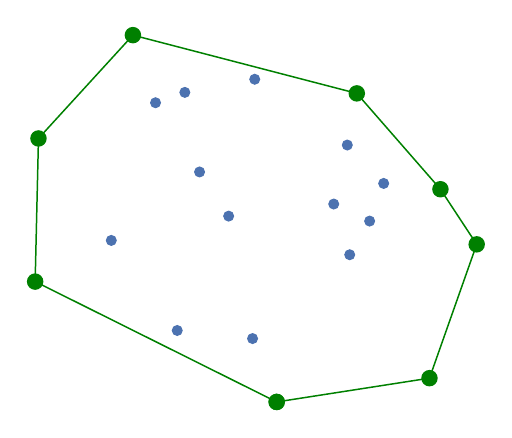
\begin{tikzpicture}[scale=0.9]

\definecolor{darkslategray38}{RGB}{38,38,38}
\definecolor{green}{RGB}{0,128,0}
\definecolor{lightgray204}{RGB}{204,204,204}
\definecolor{steelblue76114176}{RGB}{76,114,176}

\begin{axis}[
axis line style={lightgray204},
hide x axis,
hide y axis,
tick align=outside,
x grid style={lightgray204},
xmajorticks=false,
xmin=0.0669367338947019, xmax=0.894111789939664,
xtick style={color=darkslategray38},
y grid style={lightgray204},
ymajorticks=false,
ymin=-0.0362471743023485, ymax=1.03274876525929,
ytick style={color=darkslategray38}
]
\addplot [draw=steelblue76114176, fill=steelblue76114176, mark=*, only marks]
table{%
x  y
0.346517060199814 0.201667385571862
0.110198245014805 0.710446973195645
0.674196381095166 0.49152149407659
0.30956117598126 0.80506608165215
0.271019344924566 0.98415804073376
0.636154602711755 0.693008958661624
0.384544745815431 0.621686927298183
0.613069361293463 0.536676532843469
0.515872695614497 0.0123435502231805
0.856512923755802 0.429885536698643
0.794765500051758 0.575905243509799
0.104535600078564 0.331190264339077
0.698107527894101 0.591287819523784
0.652331867510728 0.829843579751645
0.776100950068952 0.0753407526360956
0.359461819254946 0.832493157115646
0.234215740614521 0.440279847038206
0.474800803395323 0.180277096021146
0.478504950884847 0.867281705269675
0.434092000130053 0.504691515965982
0.640277876553855 0.402360080889356
};
\addplot [semithick, green, mark=*, mark size=3, mark options={solid}]
table {%
0.515872695614497 0.0123435502231805
0.776100950068952 0.0753407526360956
0.856512923755802 0.429885536698643
0.794765500051758 0.575905243509799
0.652331867510728 0.829843579751645
0.271019344924566 0.98415804073376
0.110198245014805 0.710446973195645
0.104535600078564 0.331190264339077
0.515872695614497 0.0123435502231805
};
\end{axis}

\end{tikzpicture}
\end{center}
\end{overprint}
\end{figure}


\end{frame}

\begin{frame}{Algoritmo de Graham}
\end{frame}

\begin{frame}{Exemplos}

  \begin{overprint}
    \begin{columns}
      \begin{column}{0.5\textwidth}
        \begin{figure}
          \includegraphics<1-2>[width=\textwidth]{./figures/introbs_pointsonly.png}
          \includegraphics<3-4>[width=\textwidth]{./figures/fishdp_pointsonly.png}
          \includegraphics<5-6>[width=\textwidth]{./figures/dog_pointsonly.png}
          \includegraphics<7-8>[width=\textwidth]{./figures/canada_pointsonly.png}
        \end{figure}
      \end{column}
      \begin{column}{0.5\textwidth}
        \begin{figure}
          \includegraphics<2>[width=\textwidth]{./figures/introbs.png}
          \includegraphics<4>[width=\textwidth]{./figures/fishdp.png}
          \includegraphics<6>[width=\textwidth]{./figures/dog.png}
          \includegraphics<8>[width=\textwidth]{./figures/canada.png}
        \end{figure}
      \end{column}
    \end{columns}
  \end{overprint}

\end{frame}

\begin{frame}[fragile]{Selection Sort}                                                                                                                 
  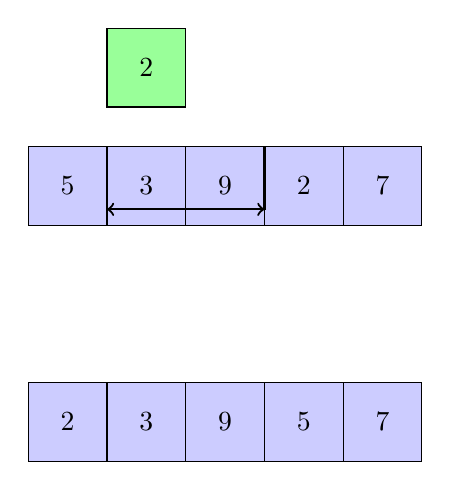
\begin{tikzpicture}                                                                                                                                    
                                                                                                                                                        
    % Lista inicial                                                                                                                                        
    \foreach \x/\num in {1/5, 2/3, 3/9, 4/2, 5/7} {                                                                                                        
      \draw[fill=blue!20] (\x,0) rectangle ++(1,1) node[midway] {\num};                                                                                    
    }                                                                                                                                                      
                                                                                                                                                           
    % Destaque da iteração atual                                                                                                                           
    % \draw[fill=yellow!60] (1,0) rectangle ++(1,1);                                                                                                         
    % \draw[fill=yellow!60] (4,0) rectangle ++(1,1);                                                                                                         
                                                                                                                                                           
    % Min valor                                                                                                                                            
    \draw[fill=green!40] (2,1.5) rectangle ++(1,1) node[midway] {2};                                                                                       
                                                                                                                                                           
    % Flechas de troca                                                                                                                                     
    \draw[->,thick] (2,1) -- ++(0,-0.8) -- ++(2,0);                                                                                                        
    \draw[->,thick] (4,1) -- ++(0,-0.8) -- ++(-2,0);                                                                                                       
                                                                                                                                                           
    % Lista após a iteração                                                                                                                                
    \foreach \x/\num in {1/2, 2/3, 3/9, 4/5/, 5/7} {                                                                                                       
      \draw[fill=blue!20] (\x,-3) rectangle ++(1,1) node[midway] {\num};                                                                                   
    }                                                                                                                                                      
                                                                                                                                                           
    \end{tikzpicture}
\end{frame}                                                                                                                                            
                                                                                                                                                         
  \begin{frame}[fragile]{Insertion Sort}                                                                                                                 
  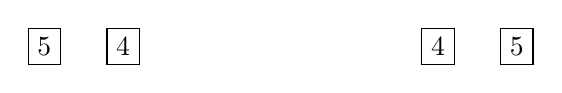
\begin{tikzpicture}[scale=1]                                                                                                                           
      \node[draw] at (0,0) {5};                                                                                                                          
      \node[draw] at (1,0) {4};                                                                                                                          
                                                                                                                                                         
      \node[draw] at (5,0) {4};                                                                                                                          
      \node[draw] at (6,0) {5};                                                                                                                          
  \end{tikzpicture}                                                                                                                                      
                                                                                                                                                         
  Insertion sort: \verb|[5, 4]| $\rightarrow$ \verb|[4, 5]|                                                                                              
  \end{frame}                                                                                                                                            
                                                                                                                                                         
  \begin{frame}[fragile]{Merge Sort}                                                                                                                     
  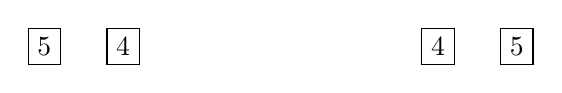
\begin{tikzpicture}[scale=1]                                                                                                                           
      \node[draw] at (0,0) {5};                                                                                                                          
      \node[draw] at (1,0) {4};                                                                                                                          
                                                                                                                                                         
      \node[draw] at (5,0) {4};                                                                                                                          
      \node[draw] at (6,0) {5};                                                                                                                          
  \end{tikzpicture}                                                                                                                                      
                                                                                                                                                         
  Merge sort: \verb|[5, 4]| $\rightarrow$ \verb|[4, 5]|                                                                                                  
  \end{frame}                                                                                                                                            
                                                                                                                                                         
  \begin{frame}[fragile]{Quick Sort}                                                                                                                     
  
\begin{tikzpicture}[scale=1]                                                                                                                           
      \node[draw] at (0,0) {5};                                                                                                                          
      \node[draw] at (1,0) {1};                                                                                                                          
      \node[draw] at (2,0) {4};                                                                                                                          
                                                                                                                                                         
      \node[draw] at (5,0) {1};                                                                                                                          
      \node[draw] at (6,0) {5};                                                                                                                          
      \node[draw] at (7,0) {4};                                                                                                                          
  \end{tikzpicture}                                                                                                                                      
                                                                                                                                                         
  Quick sort: \verb|[5,1,4]| $\rightarrow$ \verb|[1,5,4]|                                                                                                
  \end{frame}     

\begin{frame}
\frametitle{Tempo de execução}
% Two columns
\begin{columns}
  \begin{column}{0.4\textwidth}
  \begin{itemize}
    \item Pontos gerados aleatoriamente dentro de um círculo de raio 1
    \item $h \sim \sqrt{n}$, onde h é o número de vértices do fecho convexo.
  \end{itemize}
  \end{column}
  \begin{column}{0.6\textwidth}
    \begin{figure}
      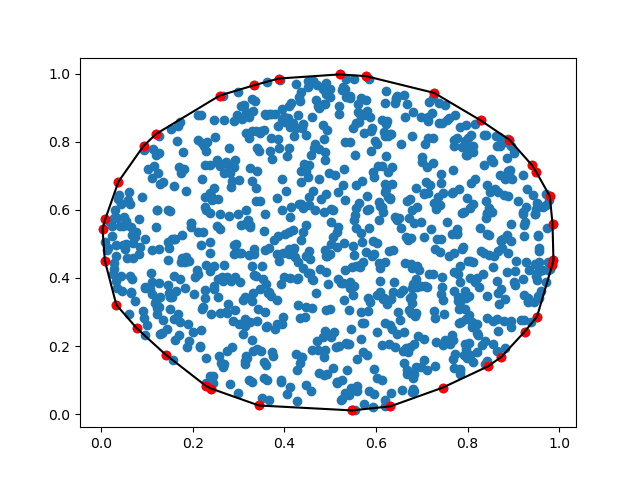
\includegraphics[width=0.9\textwidth]{./figures/random_merge_1000_1.png}
    \end{figure}
  \end{column}
\end{columns}
  
\end{frame}

\begin{frame}
\frametitle{Tempo de execução}
    \begin{figure}
      % include pgf circle_times.pgf here
      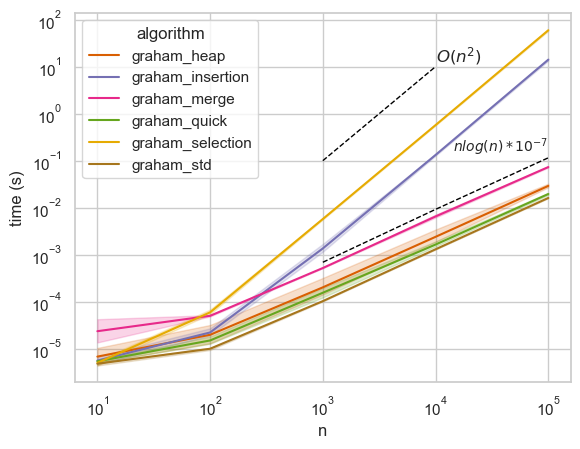
\includegraphics[width=0.9\textwidth]{./figures/circle_times.png}
    \end{figure}
\end{frame}

\end{document}
